\providecommand{\main}{..}
\documentclass[\main/main.tex]{subfiles}
\begin{document}

Minimizzo $f(x)$, con la condizione di $g_j(x) \leq 0 \forall j = 1...n $.

Supponiamo di voler identificare la posizione migliore di una discarica, e che il punto in cui i rifiuti vengono prodotti sia $R = (1,0)$, che in punto $C = (0,0)$ vi sia in una città e che si debba avere una distanza di almeno $2$ dalla città. Inoltre, la nostra discarica deve trovarsi a sinistra di $\dfrac{3}{2}$, cioè $x_0 < \dfrac{3}{2}$, perché li vi è un confine.

\begin{center}
	\begin{tikzpicture}
		% axis
		\draw[->] (-1,0) -- (3,0) node[right] {$x_1$};
		\draw[->] (0,-1) -- (0,3) node[above] {$x_2$};

		% points
		\foreach \Point/\PointLabel in {(1,0)/R, (0,0)/C}
		\draw[fill=black] \Point circle (0.05) node[above right] {$\PointLabel$};

		\draw[domain=-1:3,smooth,variable=\y,red]  plot ({3/2},{\y});
	\end{tikzpicture}
\end{center}

La funzione di minimo che vado a definire risulta:

\[
	\min f(x) = \begin{cases}
		(x_1-1)^2 + x_2^2 \\
		x_1^2 + x_2^2 = 4 \\
		x_1  < \dfrac{3}{2}
	\end{cases}
\]

\begin{figure}
	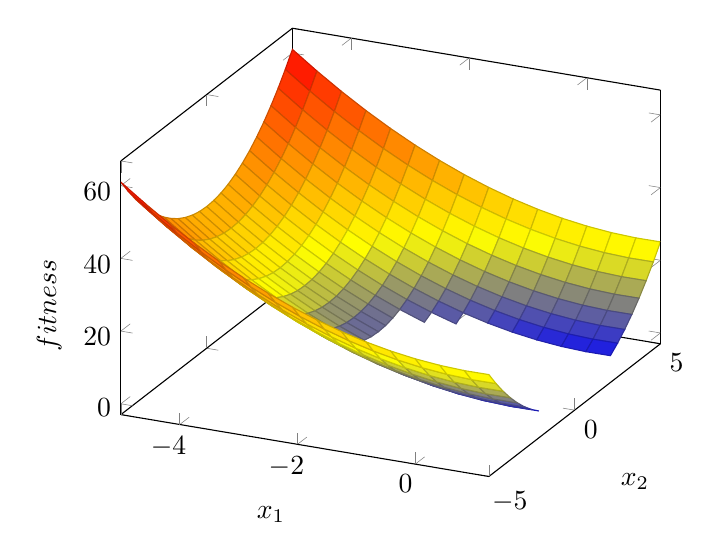
\begin{tikzpicture}
		\begin{axis}[
				xlabel=$x_1$,
				ylabel=$x_2$,
				zlabel=$fitness$
			]

			\addplot3[surf, unbounded coords=jump]
			{x^2 + y^2 > 4 && x < 3/2 ? (x-1)^2 + y^2 : NaN};

		\end{axis}
	\end{tikzpicture}
\end{figure}


\section{Programmazione matematica}

\begin{definition}{Ottimo locale}
	$\widetilde{x}$ ottimo locale $\Leftrightarrow$ $f(x) \geq f(\widetilde(x)) \forall x \in \mathbb{U}_{\widetilde{x}, \epsilon}$
\end{definition}

Dato $\widetilde{x}$ come un \textbf{ottimo locale}, e $\xi(\alpha)$ un \textbf{arco ammissibile} con la caratteristica di:

\[
	\xi(0) = \widetilde{x} \qquad
	\xi(alpha) \in X \forall \alpha \in [0, \widehat{\alpha})
\]

Allora vale che $\xi$ risulta \textbf{non migliorante}:

\[
	f(\xi(\alpha)) \geq f(\widetilde{x}) = f(\xi(0)) \forall \alpha \in [0, \widehat{\alpha})
\]

La formula sovra riportata può essere espressa più semplicemente tramite:

\[
	[\nabla f(\widetilde{x})]^T P_{\xi} \geq \emptyset
\]

\begin{definition}[Punti non regolari]
	\[
		\widetilde{x} \text{ regolare } \Leftrightarrow \nabla g_j (\widetilde{x}) \text{per $ g_j$ attivo, con le varie funzioni $g_j$ linearmente indipendenti}
	\]
\end{definition}

\begin{definition}[Punti non regolari]
	Sono dei punti per cui non vale
	\[
		[\nabla g_j (\widetilde)]^T P_\xi (\widetilde{x}) \geq 0 \text{ per $g_j$ attivo } \Leftarrow 	\begin{cases}
			\xi \text{ arco ammissibile} \\
			\widetilde{x} \text{ ottimo locale}
		\end{cases}
		\Rightarrow
		[\nabla f(\widetilde{x})]^T P_{\xi} \geq \emptyset
	\]
\end{definition}

\begin{figure}
	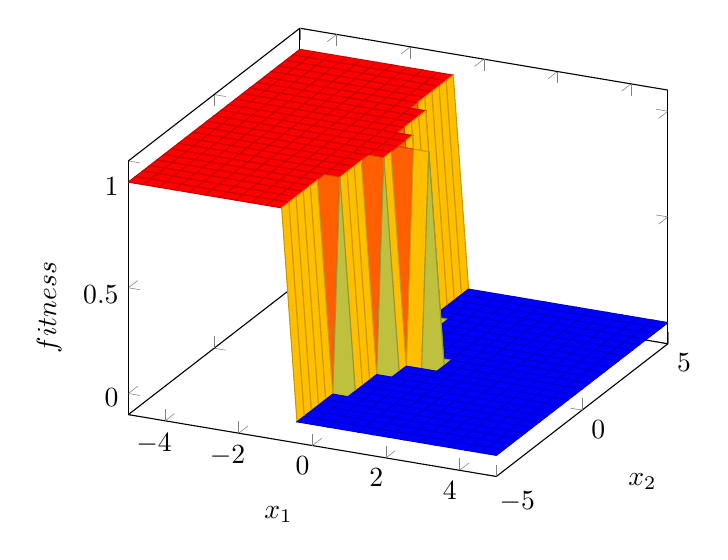
\begin{tikzpicture}
		\begin{axis}[
				xlabel=$x_1$,
				ylabel=$x_2$,
				zlabel=$fitness$
			]

			\addplot3[surf, unbounded coords=jump]
			{(x-1)^3+y<0 && ((x-1)^3-y<0)? 1 : 0};

		\end{axis}
	\end{tikzpicture}
\end{figure}

\section{Lemma di Farkas}

\begin{figure}[H]
	\[
		C_j = \{ p \in \mathbb{R}^2: g_j^T p \leq 0 \forall j \}
	\]
	\caption{Cono direzioni "opposte" ai vettori $g_j$}
\end{figure}

\begin{figure}[H]
	\[
		C_f = \{ p \in \mathbb{R}^2: f^T p \leq 0 \forall j \}
	\]
	\caption{Cono direzioni "opposte" a $f$}
\end{figure}

Se $\exists \mu_j \geq 0 : f = \sum_j \mu_j g_j \Leftrightarrow (C_g \subseteq C_f) -f^Tp \leq 0 \forall p: g_j^Tp \leq 0 \forall j$

Posso riscrivere questa formula usando i gradienti:

Se $\exists \mu_j \geq 0 : \nabla f = \sum_j \mu_j \nabla g_j \Leftrightarrow (C_g \subseteq C_f) -\nabla f^Tp \leq 0 \forall p: \nabla g_j^Tp \leq 0 \forall j$

che cosa è la combinazione lineare? e convessa? e conica?

\section{Condizioni di Karush–Kuhn–Tucker (KKT)}

Se $\widetilde(x)$ è un \textbf{ottimo locale} e \textbf{regolare}, allora $\exists \mu_j \geq 0: \nabla f(\widetilde{x}) + \sum_{j:g_j \text{ attivo}} \mu_j \nabla g_j = \emptyset$

Questo viene posto a sistema con $\mu_j g_j (\widetilde{x}) = \emptyset \forall j = 1...n$:

\[
	\begin{cases}
		\exists \mu_j \geq 0: \nabla f(\widetilde{x}) + \sum_{j:g_j \text{ attivo}} \mu_j \nabla g_j = \emptyset \\
		\mu_j g_j (\widetilde{x}) = \emptyset \forall j = 1...n                                                  \\
		g_j(\widetilde{x}) <0 \Rightarrow \mu_j =0                                                               \\
		g_j(x) \leq 0 \forall j = 1...m
	\end{cases}
\]

\section{Metodo dei vincoli}
Dato un punto $x^*$ \textbf{globalmente paretiano} per $\begin{cases}
		\min f_1 \\
		\vdots   \\
		\min f_p \\
	\end{cases} \Rightarrow x^*$ è un \textbf{ottimo globale} per $f_l(x)$, cioè vale che $f_l(x) \leq \epsilon_l = f_l(x^*)$ con $x \in X$

\section{Metodo Lessicografico}
\begin{enumerate}
	\item Si chiede al \textbf{decisore} di introdurre un \textbf{ordinamento totale} sugli indicatori, cioè ${1, \dots, P}\leadsto{\pi_1, \dots, \pi_P}$, dove $\pi_1$ viene considerato \textbf{l'indicatore principale}.
	\item Vado a selezionare tutti i \textbf{cammini a costo minimo}, limitandomi all'indicatore principale: $\min_{x \in X} f_{\pi_1} \rightarrow X_1^*$
	\item Continuo a cercare i cammini a costo minimo degli indicatori successivi, sino a che rimango con un'unica soluzione minimante valida. Se arrivo all'ultimo indicatore con più di una soluzione ne scelgo una a caso. La soluzione così ottenuta è \textbf{globalmente paretiana} (benchè tendenzialmente molto squilibrata e che non da un compromesso) perchè è un ottimo per tutte le funzioni.
\end{enumerate}

\section{Metodo lessicografico con livelli di aspirazione}
In aggiunta al passaggio preliminare visto precedentemente fisso i \textbf{livelli di aspirazione} $\epsilon_l \quad \forall l \not = \pi_1$

\section{Metodo del punto utopia}
Viene aggiunto un punto che viene descritto dal decisore come il migliore possibile, ignorando temporaneamente i vincoli, e si va quindi ad identificare una regione paretiana come quella che ne minimizza la distanza.

\begin{figure}[H]
	\centering
	\includegraphics[width=0.5\textwidth]{\main/images/utopia.jpg}
	\caption{Metodo del punto utopia}
\end{figure}

\end{document}